%%%%%%%%%%%%%%%%%%%%%%%%%%%%%%%%%%%%%%%%%%%%%%%%%%%%%%%%%%%%%%%%%%%%%%%%%%%%%%%
%                         File: osa-revtex4-1.tex                             %
%                        Date: April 15, 2013                                 %
%                                                                             %
%                              BETA VERSION!                                  %
%                   JOSA A, JOSA B, Applied Optics, Optics Letters            %
%                                                                             %
%            This file requires the substyle file osajnl4-1.rtx,              %
%                   running under REVTeX 4.1 and LaTeX 2e                     %
%                                                                             %
%                   USE THE FOLLOWING REVTeX 4-1 OPTIONS:                     %
% \documentclass[osajnl,twocolumn,showpacs,superscriptaddress,10pt]{revtex4-1}%
%                    %% Use 11pt for Applied Optics                           %
%                                                                             %
%               (c) 2013 The Optical Society of America                       %
%                                                                             %
%%%%%%%%%%%%%%%%%%%%%%%%%%%%%%%%%%%%%%%%%%%%%%%%%%%%%%%%%%%%%%%%%%%%%%%%%%%%%%%

\documentclass[osajnl,twocolumn,showpacs,superscriptaddress,10pt]{revtex4-1} %% use 11pt for Applied Optics
%\documentclass[osajnl,preprint,showpacs,superscriptaddress,11pt]{revtex4-1} %% use 12pt for preprint option
\usepackage{amsmath,nccmath,amssymb,graphicx,float,minted,xparse,tikz}
\usepackage[utf8]{inputenc}
\graphicspath{{images/}}

\usepackage{mathtools,enumitem}
\usepackage{minted}

\begin{document}

\title{Programación Distribuida y Tiempo Real}

\author{Ulises Jeremias Cornejo Fandos}
\affiliation{Licenciatura en Informática, Facultad de Informática, UNLP}

\maketitle %% required

\section{Para los ejemplos de RPC proporcionados (*.tar, analizar en el orden dado a los nombres de
los archivos):}

\subsection{Mostrar cómo serían los mismos procedimientos si fueran locales, es decir haciendo el
proceso inverso del realizado en la clase de explicación de RPC.}

Si los procesos fueran todos locales, la programación de los mismos resultaria en una compilación de uno o más ".c" con una única función \textit{main} y un único binario ejecutable. En el ejemplo provisto se puede observar como todo el código del programa se encuentra en un único ".c", como se describe anteriormente.

En este caso no habría latencia en la comunicación dado que no existiría tal comunicacón. Al no definirse un modelo cliente/servidor, ya no existiría una comunicación entre hosts y todos los llamados a funciones se realizarían en el mismo espacio de direcciones.

\subsection{Ejecutar los procesos y mostrar la salida obtenida (del “cliente” y del “servidor”) en cada
uno de los casos.}

Las capturas se muestran a continuación:

\subsubsection{Simple}

\begin{figure}[H]
    \centering
    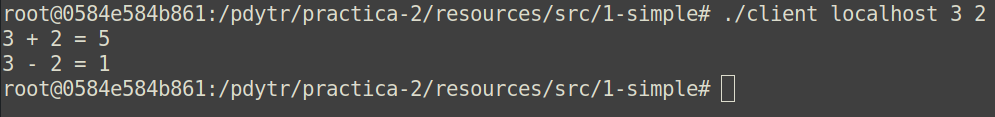
\includegraphics[width=0.5\textwidth]{capturas/1-simple-client}
    \caption{Salida de la ejecución del cliente dados los parámetros \textit{localhost}, \textit{3} y \textit{2}}.
    \label{figure:1-simple-client}
\end{figure}

\begin{figure}[H]
    \centering
    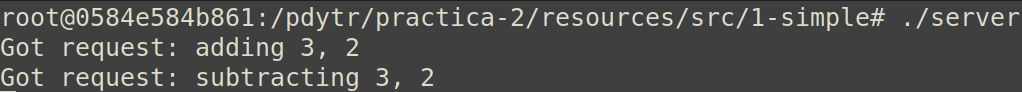
\includegraphics[width=0.5\textwidth]{capturas/1-simple-server}
    \caption{Salida de la ejecución del servidor.}
    \label{figure:1-simple-server}
\end{figure}

\subsubsection{U1}

La ejecución del servidor no tiene salida al momento de resolver una consulta del cliente.

\begin{figure}[H]
    \centering
    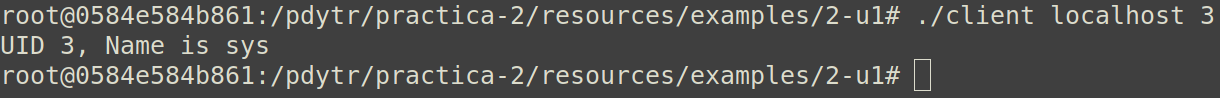
\includegraphics[width=0.5\textwidth]{capturas/2-u1-client}
    \caption{Salida de la ejecución del cliente dados los parámetros \textit{localhost} y \textit{3}}.
    \label{figure:2-u1-client}
\end{figure}

\subsubsection{Array}

\begin{figure}[H]
    \centering
    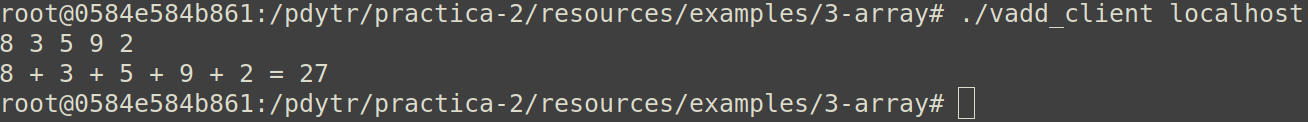
\includegraphics[width=0.5\textwidth]{capturas/3-array-client}
    \caption{Salida de la ejecución del cliente dados los parámetros \textit{localhost}, $8$, $3$, $5$, $9$ y $2$}.
    \label{figure:3-array-client}
\end{figure}

\begin{figure}[H]
    \centering
    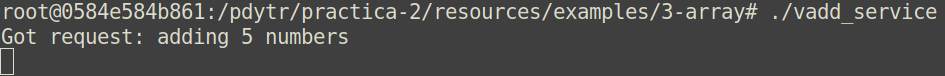
\includegraphics[width=0.5\textwidth]{capturas/3-array-server}
    \caption{Salida de la ejecución del servidor.}
    \label{figure:3-array-server}
\end{figure}

\subsubsection{List}

La ejecución del servidor no tiene salida al momento de resolver una consulta del cliente.

\begin{figure}[H]
    \centering
    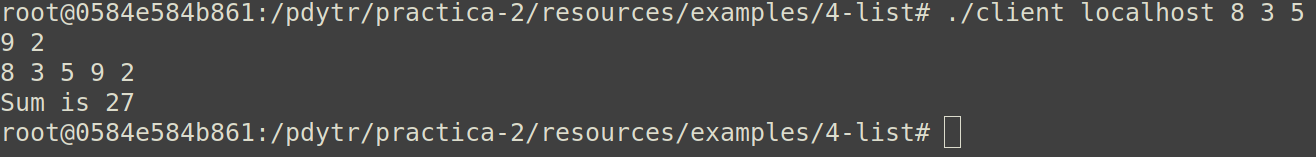
\includegraphics[width=0.5\textwidth]{capturas/4-list-client}
    \caption{Salida de la ejecución del cliente dados los parámetros \textit{localhost}, $8$, $3$, $5$, $9$ y $2$}.
    \label{figure:4-list-client}
\end{figure}

\subsection{Mostrar experimentos donde se produzcan errores de conectividad del lado del cliente y
del lado del servidor. Si es necesario realice cambios mínimos para, por ejemplo, incluir
sleep() o exit(), de forma tal que no se reciban comunicaciones o no haya receptor para
las comunicaciones. Verifique con UDP y con TCP.}

En ambos casos se modifica la implementación de la función \mintinline{c}{int *add_1_svc(operands *argp, struct svc_req *rqstp);} en el archivo \textit{simpservice.c}. Es decir, la implementación del proceso servidor, agregando un sleep o exit, según corresponda, respectivamente.

\subsubsection{UDP}
  Agregando un llamado a la función \textbf{exit}, el proceso servidor termina en medio de la operación, (\textit{ver fig. \ref{figure:1-simple-server-udp-exit}}) por lo que el cliente termina la comunicación cuando finaliza el timeout definido en su proceso, (\textit{ver fig. \ref{figure:1-simple-client-udp-exit}}).
  
  Lo mismo pasa si el servidor tarda mucho en procesar lo pedido y responder, cosa que se simula agregando un llamadao a la función \textbf{sleep} dentro del proceso servidor. Cuando el sleep tiene una duración mayor a la del timeout definido en el cliente, el servidor no da su respuesta antes del timeout y el cliente cierra la conexión, (\textit{ver fig. \ref{figure:1-simple-client-udp-sleep}}). En este caso, el servidor continuará su ejecución esperando el proximo request, (\textit{ver fig. \ref{figure:1-simple-server-udp-sleep}}).
  
\begin{figure}[H]
    \centering
    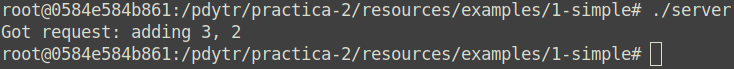
\includegraphics[width=0.5\textwidth]{capturas/1-simple-server-udp-exit}
    \caption{Salida de la ejecución del service utilizando UDP y la función exit.}.
    \label{figure:1-simple-server-udp-exit}
\end{figure}

\begin{figure}[H]
    \centering
    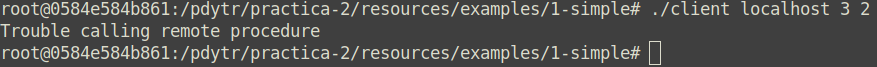
\includegraphics[width=0.5\textwidth]{capturas/1-simple-client-udp-exit}
    \caption{Salida de la ejecución del cliente utilizando UDP.}.
    \label{figure:1-simple-client-udp-exit}
\end{figure}

\begin{figure}[H]
    \centering
    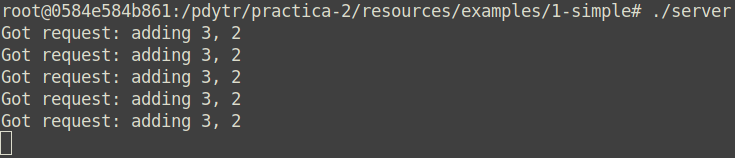
\includegraphics[width=0.5\textwidth]{capturas/1-simple-server-udp-sleep}
    \caption{Salida de la ejecución del service utilizando UDP y la función sleep.}.
    \label{figure:1-simple-server-udp-sleep}
\end{figure}

\begin{figure}[H]
    \centering
    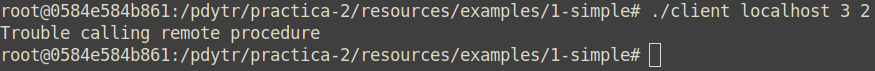
\includegraphics[width=0.5\textwidth]{capturas/1-simple-client-udp-sleep}
    \caption{Salida de la ejecución del cliente utilizando UDP.}.
    \label{figure:1-simple-client-udp-sleep}
\end{figure}

\subsection{TCP}

El resultado es exactamente el mismo que el descripto anteriormente en el caso de UDP, cuando el servidor termina cuando se agrega el \textbf{exit}, (\textit{ver figs. \ref{figure:1-simple-server-tcp-exit} y \ref{figure:1-simple-client-tcp-exit}}) y cuando tarda mas de lo debido con la función \textbf{sleep}, (\textit{ver figs. \ref{figure:1-simple-server-tcp-sleep} y \ref{figure:1-simple-client-tcp-sleep}}).

\begin{figure}[H]
    \centering
    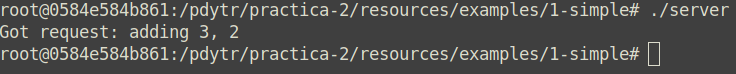
\includegraphics[width=0.5\textwidth]{capturas/1-simple-server-tcp-exit}
    \caption{Salida de la ejecución del service utilizando TCP y la función exit.}.
    \label{figure:1-simple-server-tcp-exit}
\end{figure}

\begin{figure}[H]
    \centering
    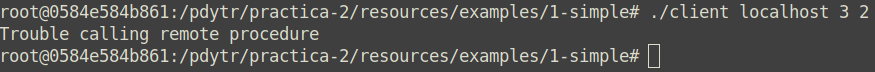
\includegraphics[width=0.5\textwidth]{capturas/1-simple-client-tcp-exit}
    \caption{Salida de la ejecución del cliente utilizando TCP.}.
    \label{figure:1-simple-client-tcp-exit}
\end{figure}

\begin{figure}[H]
    \centering
    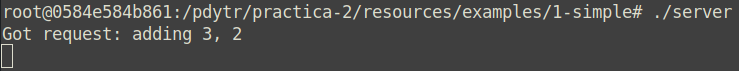
\includegraphics[width=0.5\textwidth]{capturas/1-simple-server-tcp-sleep}
    \caption{Salida de la ejecución del service utilizando TCP y la función sleep.}.
    \label{figure:1-simple-server-tcp-sleep}
\end{figure}

\begin{figure}[H]
    \centering
    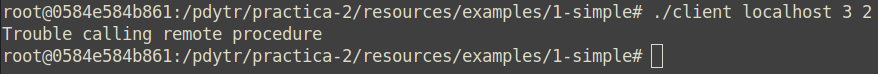
\includegraphics[width=0.5\textwidth]{capturas/1-simple-client-tcp-sleep}
    \caption{Salida de la ejecución del cliente utilizando TCP.}.
    \label{figure:1-simple-client-tcp-sleep}
\end{figure}

\section{Describir/analizar las opciones a) - N b) -M y - A, verificando si se pueden utilizar estas opciones y comentar que puede ser necesario para tener procesamiento concurrente del “lado del cliente” y del “lado del servidor” con la versión
utilizada de rpcgen. Una lista completa de opciones se describe en
http://download.oracle.com/docs/cd/E19683-01/816-1435/rpcgenpguide-1939/index.html}

\subsection{}
El flag -N intenta de generar código en un estándar más nuevo que el ANSI (flag -C).
Al intentar compilar el código con ese flag, utilizando el código original, falla.
Esto se debe a que rcpgen, genera un .h las funciones con el tipo SIN puntero, a diferencia del flag -C, que los genera como punteros a operand.

\subsection{}
El flag -M sirve para generar código seguro para la concurrencia, utilizando un paŕametro extra al servicio, de tipo int *. \\
El flag -A, es la configuracion por default, que dependiendo el sistema en el que se compila, va a ser (o no), seguro para la concurrencia multihilo.

\section{Analizar la transparencia de RPC en cuanto al manejo de parámetros de los procedimientos
remotos. Considerar lo que sucede en el caso de los valores de retorno. Puede aprovechar los
ejemplos provistos.}

rpcgen utiliza la estructura definida en el archivo ".x" para generar estructuras C en ambos puntos (cliente y servidor), con las cuales va a trabajar casteando. \\

El servicio recibe punteros a estas estructuras, las cuales va a trabajar y retornar nuevamente casteando a (caddr\_t), el cual es equivalente a un \mintinline{c}{void *}.

Esto nos permite trabajar con cualquier tipo de C, siempre volviendo a castear a la estructura definida a partir del ".x".

\section{Con la finalidad de contar con una versión muy restringida de un sistema de archivos remoto, en el cual se puedan llevar a cabo las operaciones enunciadas informalmente como:}

\begin{itemize}
  \item \textbf{leer}: dado un nombre de archivo, una posición y una cantidad de bytes a leer, retorna 1) los bytes efectivamente leídos desde la posición pedida y la cantidad pedida en caso de ser posible, y 2) la cantidad de bytes que efectivamente se retornan leídos.
  
  \item \textbf{escribir}: dado un nombre de archivo, una cantidad de bytes determinada, y un buffer a partir del cual están los datos, se escriben los datos en el archivo dado. Si el archivo existe, los datos se agregan al final, si el archivo no existe, se crea y se le escriben los datos. En todos los casos se retorna la cantidad de bytes escritos.
\end{itemize}


\subsection{Defina e implemente con RPC un servidor. Documente todas las decisiones tomadas.}

\subsection{Implemente un cliente RPC del servidor anterior que copie un archivo del sistema de
archivos del servidor en el sistema de archivos local y genere una copia del mismo archivo
en el sistema de archivos del servidor. En todos los casos se deben usar las operaciones
de lectura y escritura del servidor definidas en el item anterior, sin cambios específicos
del servidor para este item en particular. Al finalizar la ejecución del cliente deben quedar
tres archivos en total: el original en el lado del servidor, una copia del original en el lado
del cliente y una copia en el servidor del archivo original. El comando diff no debe
identificar ninguna diferencia entre ningún par de estos tres archivos.}

Para este punto, se implementaron las funciones básicas, \texttt{write}, \texttt{read} y \texttt{list}

Como primera instancia, se define el archivo \texttt{.x} de la siguiente forma:

\inputminted[mathescape]{c}{../resources/src/5-ftp/ftp.x}

Se busco manejar cualquier tipo de archivos, por eso el uso del tipo opaque.

Luego se definieron el cliente junto a los comandos disponibles.

Con el objetivo de mejorar la legibilidad del codigo, se opto por utilizar un arreglo de estructuras con punteros a funciones para diferenciar rapidamente los comandos.

El parseo de los argumentos al cliente cuenta con 2 etapas, la primera busca algun comando valido, y se realiza a recorriendo manualmente \texttt{argv}. \\
La segunda busca las flags posibles para los comandos, esto se hizo usando la libreria \texttt{getopt} para mayor facilidad.

La conexion con el servidor tuvo que ser obligatoriamente del tipo \textbf{TCP} para soportar los grandes volumenes de datos.


\section{Timeouts en RPC:}

\subsection{Desarrollar un experimento que muestre el timeout definido para las llamadas RPC y el
promedio de tiempo de una llamada RPC.}

Para el experimento del timeout usaremos el caso 1-simple. 
Vemos que si ponemos en el proceso servidor un delay de 25 mediante un sleep(25) en el medio de la comunicación:

Entonces la comunicación se realiza exitosamente y la llamada al proceso remoto termina de forma correcta.

En cambio si ponemos en el proceso servidor un delay de 26 mediante un sleep(26) en el medio de la comunicación.

Entonces la comunicación se corta por parte del cliente y la llamada no se completa. (\textit{Ver fig. \ref{figure:6-sleep-timeout-25}}).

Mediante estos resultados podemos afirmar que el timeout definido en el proceso cliente es el 25 segundos, por los que si el proceso servidor o la comunicación tardan más de ese tiempo entonces el cliente finalizará la comunicación abruptamente dando por sentado una falla en la misma.

\begin{figure}[H]
    \centering
    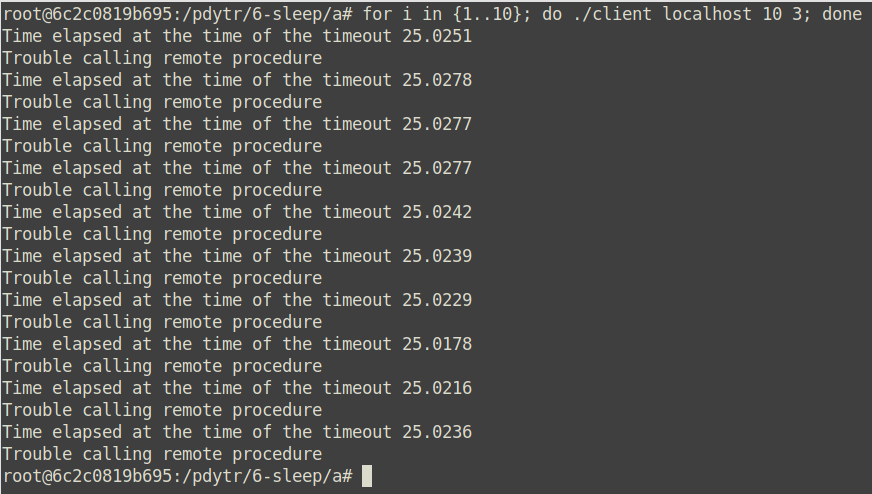
\includegraphics[width=0.5\textwidth]{capturas/6-sleep-timeout-25}
    \caption{Tiempos de ejecución calculados al momento de alcanzar el timeout}.
    \label{figure:6-sleep-timeout-25}
\end{figure}

\subsection{Reducir el timeout de las llamadas RPC a un 10\% menos del promedio encontrado
anteriormente. Mostrar y explicar el resultado para 10 llamadas.}

Luego de enviar una solicitud al servidor, un proceso cliente espera un período default de 25 segundos para recibir una respuesta. Este valor puede ser modificado utilizando la rutina \mintinline{c}{clnt_control()}.

Usando una estructura timeval, se puede configurar los segundos que se deseen para el timeout del cliente se la siguiente forma:

\begin{minted}{c}
struct timeval tv;
CLIENT *clnt;

tv.tv_sec = 60;	
tv.tv_usec = 0;

clnt_control(clnt, CLSET_TIMEOUT, &tv);
\end{minted}


Teniendo en cuenta esto, se prueba con un timeout de 10 segundos, realizando el experimento anterior nuevamente 10 veces obteniendo el siguiente resultado. (\textit{Ver fig. \ref{figure:6-sleep-timeout-10}}).

\begin{figure}[H]
    \centering
    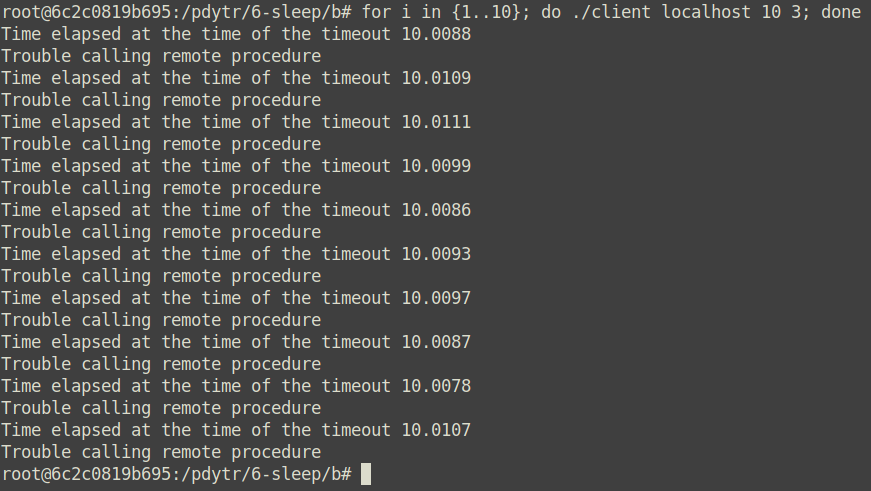
\includegraphics[width=0.5\textwidth]{capturas/6-sleep-timeout-10}
    \caption{Tiempos de ejecución calculados al momento de alcanzar el timeout}.
    \label{figure:6-sleep-timeout-10}
\end{figure}


\subsection{Desarrollar un cliente/servidor RPC de forma tal que siempre se supere el tiempo de
timeout. Una forma sencilla puede utilizar el tiempo de timeout como parámetro del
procedimiento remoto, donde se lo utiliza del lado del servidor en una llamada a sleep(),
por ejemplo.}

En la estructura cliente/servidor generada, se recibe como argumento un tiempo el cual define el timeout del cliente y se envia al servidor para que este haga un sleep con el cuadrado de ese tiempo para que siempre se genere un timeout.


\end{document}
